\section{Slobodni binarni dijagrami odlu\v{c}ivanja (FBDD)}
\label{sec:FBDD}

Slobodni binarni dijagrami odlu\v{c}ivanja (engl. \emph{Free Binary Decision Diagrams} \cite{FBDD}, u daljem tekstu \emph{FBDD}) koriste \v{S}enonovu dekompoziciju u svakom \v{c}voru (sli\v{c}no kao kod OBDD) ali se du\v{z} razli\v{c}itih putanja mogu koristiti razli\v{c}ita uredjenja. \v{S}tavi\v{s}e, svaka promenljiva se sme testirati samo jednom. Ukoliko se promenljive biraju istim redosledom du\v{z} svih putanja, rezultat je OBDD. Drugim re\v{c}ima, OBDD su specijalan slu\v{c}aj FBDD. Iako nisu u op\v{s}tem slu\v{c}aju kanoni\v{c}ka struktura, uz modifikacije je mogu\'c{}e posti\'c{}i kanoni\v{c}nost. \v{S}tavi\v{s}e, FBDD se efikasno minimizuju i izlistavaju.

Dokazano je  postojanje funkcija koje se mogu efikasno predstaviti pomo\'c{}u FBDD (u polinomijalnom prostoru), dok je za OBDD u najgorem slu\v{c}aju potreban eksponencijalan broj \v{c}vorova. Glavni problem je nepostojanje efikasne heuristike za odabir redosleda promenljivih. Iako postoji dosta pristupa za re\v{s}avanje pomenutog problema \cite{FBDD}, nije pronadjeno zna\v{c}ajno br\v{z}e unapredjenje u odnosu na OBDD.

SAT re\v{s}ava\v{c}i se mogu koristiti za konstrukciju i minimizaciju FBDD. SAT re\v{s}ava\v{c}i se mogu shvatiti kao pretra\v{z}iva\v{c}i binarnog stabla odlu\v{c}ivanja za datu funkciju. U op\v{s}tem slu\v{c}aju, uz fiksni izbor odabira promenljivih u implementaciji SAT re\v{s}ava\v{c}a, drvo koje SAT re\v{s}ava\v{c} pretra\v{z}uje je zapravo OBDD. U slu\v{c}aju nedeterministi\v{c}kog izbora promenljivih, to drvo je FBDD.

U nastavku se podrazumeva da je \v{c}italac upoznat sa terminima iskazne logike. Prvo \'c{}emo, uz kori\v{s}\'c{}enje SAT re\v{s}ava\v{c}a, opisati proces konstrukcije FBDD (deo \ref{subsec:FBDDConstructionViaSAT}), a zatim proces minimizacije FBDD (deo \ref{subsec:FBDDMinimization}).


\subsection{Konstrukcija FBDD uz pomo\'c{} SAT re\v{s}ava\v{c}a}
\label{subsec:FBDDConstructionViaSAT}

SAT re\v{s}ava\v{c}i pronalaze valuaciju $v$ takvu da je $f(v) = 1$ za datu funkciju $f$, ili pokazuju nepostojanje takvog $v$. Tokom procesa pretrage valuacija, prave se razni izbori i implikacije. Posmatranjem procesa pronala\v{z}enja pomenute valuacije mo\v{z}emo definisati osnovne osobine koje proces konstrukcije FBDD mora da ispunjava:

\begin{obsn}
    Neka je data bulovska funkcija $f : \mathbb{B}^{n} \rightarrow \mathbb{B}$  u KNF normalnoj formi. Tada va\v{z}i:
    \begin{itemize}
        \item Svaka valuacija koja zadovoljava $f$ odgovara putu koji vodi ka vrednosti $1$ u FBDD koji predstavlja $f$.
        \item Svaka konfliktna valuacija odgovara putu koji vodi ka vrednosti $0$ u FBDD koji predstavlja $f$.
        \item Svaka implikacija $x_{i} = b$, gde je $x \in f, b \in \mathbb{B}$ odgovara putu koji vodi ka vrednosti $0$ u FBDD koji predstavlja $f$. Ovaj put se moze konstruisati koriste\'c{}i trenutnu parcijalnu valuaciju $v$ uz $x_{i} = \overline{b}$.
    \end{itemize}
\end{obsn}

\begin{exmp}
    Neka je data funkcija $f(x_{1}, x_{2}, x_{3}, x_{4}) = (x_{1} \vee x_{2}) \wedge (x_{3} \vee x_{4}) \wedge (x_{1} \vee x_{2} \vee \overline{x_{4}})$. Konstrui\v{s}emo FBDD za datu funkciju $f$ posmatraju\'c{}i korake SAT re\v{s}ava\v{c}a. \v{C}itav proces je prikazan na levom dijagramu na slici \ref{diag:FBDDConstruction}.

    U po\v{c}etku re\v{s}ava\v{c} uz pomo\'c{} heuristike dodeljuje $x_{1}$ vrednost $0$ \textit{(a)}. Ovo dovodi do toga da $x_{2}$ mora imati vrednost $1$ \textit{(b)} kako bi klauza $x_{1} \vee x_{2}$ bila zadovoljena. S obzirom da smo upravo iskoristili implikaciju, zaklju\v{c}ujemo da je valuacija u kojoj je $x_{1} = 0$ i $x_{2} = 0$ konfliktna, odnosno $f(0, 0, x_{3}, x_{4}) = 0$ \textit{(c)}. U slede\'c{}em koraku sli\'c{}no kao na po\v{c}etku se bira vrednost za $x_{3}$, na primer $0$. Ovakva dodela nas dovodi do konflikta \textit{(d)}. Uzimaju\'c{}i vrednost $1$ za promenljivu $x_{3}$, sve klauze su zadovoljene bez obzira na vrednost promenljive $x_{4}$ \textit{(e)}. S obzirom da je pronadjena zadovoljavaju\'c{}a valuacija, SAT re\v{s}ava\v{c} prestaje s radom.
    \label{exmp:FBDDConstruction1}
    \qed
\end{exmp}

Kao \v{s}to je prikazano na levom delu slike \ref{diag:FBDDConstruction}, kreiran je parcijalni FBDD funkcije koriste\'c{}i SAT re\v{s}ava\v{c} koji je prona\v{s}ao jednu valuaciju u kojoj funkcija $f$ ima vrednost $1$. S obzirom da \v{z}elimo kompletni FBDD, potrebno je da istra\v{z}imo i ostale putanje (tzv. \emph{All Solution SAT}). Ovo se posti\v{z}e dodavanjem \emph{blokiraju\'c{}e klauze} u skup klauza koje SAT re\v{s}ava\v{c} poku\v{s}ava da zadovolji svaki put kad se pronadje valuacija koja zadovoljava teku\'c{}i skup klauza. U primeru \ref{exmp:FBDDConstruction1}, s obzirom da je pronadjena valuacija $\{0, 1, 1, x_{4}\}$, formira se blokiraju\'c{}a klauza $(x_{1} \vee \overline{x_{2}} \vee \overline{x_{3}})$ i pretraga se nastavlja (primer \ref{exmp:FBDDConstruction2}). Rezultat pretrage \v{c}itavog prostora vrednosti se mo\v{z}e videti na desnom delu slike \ref{diag:FBDDConstruction}.

\begin{figure}[H]
    \centering
    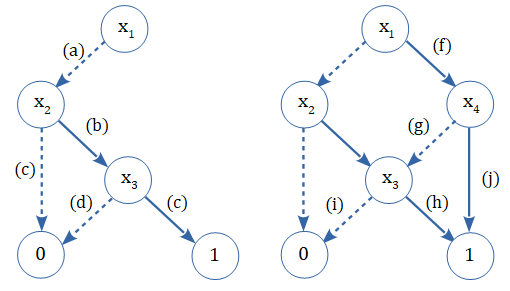
\includegraphics[scale=0.7]{slike/FBDD_Construction.PNG}
    \caption{Proces konstrukcije FBDD uz pomo\'c{} SAT re\v{s}ava\v{c}a}
    \label{diag:FBDDConstruction}
\end{figure}

\begin{exmp}
    Nastavljamo sa konstrukcijom FBDD iz primera \ref{exmp:FBDDConstruction1} dodaju\'c{}i blokiraju\'c{}u klauzu $(x_{1} \vee \overline{x_{2}} \vee \overline{x_{3}})$. Ona izaziva konflikt i povratak (engl. \emph{backtracking}) do $x_{1}$, zaklju\v{c}uju\'c{}i $x_{1} = 1$ \textit{(f)} kako bi se zadovoljila tre\'c{}a klauza. Slede\'c{}i korak je dodela $x_{4} = 0$ \textit{(g)} koja dovodi do jedne zadovoljavaju\'c{}e \textit{(h)} i jedne konfliktne valuacije \textit{(i)} zbog druge klauze. Zadovoljavaju\'c{}a valuacija se koristi kako bi se formirala blokiraju\'c{}a klauza $(\overline{x_{1}} \vee x_{3} \vee \overline{x_{4}})$. Povratkom se dolazi do $x_{4}$ i pronalazi se poslednje re\v{s}enje \textit{(j)}. S obzirom da je pretra\v{z}en ceo prostor, pretraga se zaustavlja i FBDD je konstruisan. Napomenimo da su neke grane ve\'c{} bile prisutne u dijagramu, stoga nisu zapravo dodate (koraci \textit{(h)} i \textit{(i)}).
    \label{exmp:FBDDConstruction2}
    \qed
\end{exmp}

FBDD dijagrami kreirani ovim postupkom mogu sadr\v{z}ati odredjene izomorfizme u sebi, odnosno ne moraju biti minimalni. U odeljku koji sledi \'c{}e biti vi\v{s}e re\v{c}i o identifikaciji izomorfizama i redukciji FBDD.


\subsection{Detekcija izomorfizama i minimizacija FBDD}
\label{subsec:FBDDMinimization}

FBDD dobijen postupkom opisanim u odeljku \ref{subsec:FBDDConstructionViaSAT} \v{c}esto sadr\v{z}i izomorfne pod-grafove. Za razliku od OBDD, gde se izomorfizmi mogu detektovati veoma brzo zbog fiksnog redosleda promenljivih, FBDD zbog svoje osobine nepostojanja fiksnog redosleda odabira promenljivih ne mogu da koriste iste tehnike za detekciju izomorfizama. Neke od poznatijih tehnika redukcije FBDD su \emph{odse\v{c}ne linije} (engl. \emph{cutlines}) i \emph{odse\v{c}ni skupovi} (engl. \emph{cutsets}).

Odse\v{c}ne linije se koriste nad KNF formulama dobijenim iz logi\v{c}kih kola. Ukoliko su ulazi u kolo $C$ delimi\v{c}no odredjeni, mogu\'c{}e je odrediti neke od internih signala. Skup internih signala, koji formiraju granicu sa nepoznatim signalima kola $C$, defini\v{s}e odse\v{c}nu liniju. Na implementacionom nivou se implementiraju koriste\'c{}i he\v{s}-tabele, a s obzirom da se sastoje od varijabli mogu se lako reprezentovati preko klauze (sli\v{c}no blokiraju\'c{}im klauzama opisanim u \ref{subsec:FBDDConstructionViaSAT}). Kako bi se odse\v{c}ne linije mogle primeniti u op\v{s}tem slu\v{c}aju, proces pretrage SAT re\v{s}ava\v{c}a bi se morao ograni\v{c}iti.

Odse\v{c}ni skupovi za razliku od odse\v{c}nih linija uzimaju kao ulaz KNF formulu u op\v{s}tem obliku. Deo prostora pretrage koji je ve\'c{} pretra\v{z}en se \v{c}uva kao podskup klauza u kombinaciji sa skupom promenljivih sa dodeljenom vredno\v{s}\'c{}u. Odse\v{c}ni skup je podskup inicijalnog skupa klauza. U njemu se nalaze one klauze koje sadr\v{z}e barem jedan literal kojem je dodeljena vrednost, i barem jedan literal kojem nije dodeljena vrednost, redom. Mo\v{z}e se pokazati da je za detekciju izomorfizama unutar FBDD dovoljno posmatrati odse\v{c}ni skup.

Zainteresovani \v{c}italac mo\v{z}e detaljnije opise i eksperimentalne rezultate na\'c{}i u \cite{FBDD}.
